\documentclass[a4paper, table]{article}
% Useful packages, sorted so packages of similar functionality are grouped together. Not all are essential to make the document work, however an effort was made to make this list as minimalistic as possible. Feel free to add your own!

% Essential for making this template work are graphicx, float, tabularx, tabu, tocbibind, titlesec, fancyhdr, xcolor and tikz. 

% Not essential, but you will have to debug the document a little bit when removing them are amsmath, amsthm, amssymb, amsfonts, caption, subcaption, appendix, enumitem, hyperref and cleveref.

% inputenc, lipsum, booktabs, geometry and microtype are not required, but nice to have.
\usepackage[spanish]{babel} % Agrega soporte para español
\usepackage[utf8]{inputenc} % Allows the use of some special characters
\usepackage{amsmath, amsthm, amssymb, amsfonts} % Nicer mathematical typesetting
\usepackage{lipsum} % Creates dummy text lorem ipsum to showcase typsetting 

\usepackage{graphicx} % Allows the use of \begin{figure} and \includegraphics
\usepackage{float} % Useful for specifying the location of a figure ([H] for ex.)
\usepackage{caption} % Adds additional customization for (figure) captions
\usepackage{subcaption} % Needed to create sub-figures

\usepackage{tabularx} % Adds additional customization for tables
\usepackage{tabu} % Adds additional customization for tables
\usepackage{booktabs} % For generally nicer looking tables

\usepackage[nottoc,numbib]{tocbibind} % Automatically adds bibliography to ToC
\usepackage[margin = 2.5cm]{geometry} % Allows for custom (wider) margins
\usepackage{microtype} % Slightly loosens margin restrictions for nicer spacing  
\usepackage{titlesec} % Used to create custom section and subsection titles
\usepackage{titletoc} % Used to create a custom ToC
\usepackage{appendix} % Any chapter after \appendix is given a letter as index
\usepackage{fancyhdr} % Adds customization for headers and footers
\usepackage[shortlabels]{enumitem} % Adds additional customization for itemize. 

\usepackage{hyperref} % Allows links and makes references and the ToC clickable
\usepackage[noabbrev, capitalise]{cleveref} % Easier referencing using \cref{<label>} instead of \ref{}

\usepackage{xcolor} % Predefines additional colors and allows user defined colors
\usepackage[T1]{fontenc}
\usepackage{geometry}
\usepackage{array}
\usepackage{longtable}
\usepackage{multirow}
\usepackage{wrapfig}
\usepackage{setspace}
\usepackage{pgfgantt}

\usepackage{tikz} % Useful for drawing images, used for creating the frontpage
\usetikzlibrary{positioning} % Additional library for relative positioning 
\usetikzlibrary{calc} % Additional library for calculating within tikz

% Defines a command used by tikz to calculate some coordinates for the front-page
\makeatletter
\newcommand{\gettikzxy}[3]{%
  \tikz@scan@one@point\pgfutil@firstofone#1\relax
  \edef#2{\the\pgf@x}%
  \edef#3{\the\pgf@y}%
}
\makeatother
 % Loads in the preamble 
% Give your report a title
\newcommand\reporttitle{Poneglyph MapReduce}

% Insert course code, name, quartile number and year (or any other subtitle)
\newcommand\reportsubtitle{
Tópicos Especiales en Telemática
}

% Add your group number (for DBL) or any other text.
\newcommand\groupnumber{
\textbf{Group Number: S2566-0671}
}

% Insert authors and student numbers here
\newcommand\reportauthors{
Camilo Ortegón Saugster \\
Sebastián Salazar Osorio \\
Juan Manuel Young Hoyos
}

% Add the name of your tutor (for DBL) or any other text.
\newcommand\grouptutor{
Tutor: Juan Carlos Montoya Mendoza
}

% Date and location (default: current date and Medellín)
\newcommand\placeanddate{
Medellín, \today
}

% Define EAFIT-blue (color of the EAFIT logo). Can be changed to drastically change the look of the template
\definecolor{EAFIT-blue}{RGB}{2, 8, 115}

% Sets up hyperlinks in the document to be colored
\hypersetup{
    colorlinks=true,
    linkcolor=EAFIT-blue,
    urlcolor=EAFIT-blue,
    citecolor = EAFIT-blue
    }
\urlstyle{same} % Defines settings for link and reference formatting

% Change bullet style for level 1, 2 and 3 respectively for itemize
\renewcommand{\labelitemi}{\scriptsize\textcolor{EAFIT-blue}{$\blacksquare$}}% level 1
\renewcommand{\labelitemii}{\scriptsize\textcolor{EAFIT-blue}{$\square$}}% level 2
\renewcommand{\labelitemiii}{\textcolor{EAFIT-blue}{$\circ$}}% level 3

% \renewcommand{\labelitemi}{\small\textcolor{EAFIT-blue}{\ding{70}}} % level 1
% \renewcommand{\labelitemii}{\small\textcolor{EAFIT-blue}{\ding{71}}}% level 2
% \renewcommand{\labelitemiii}{\tiny\textcolor{EAFIT-blue}{\ding{71}}}% level 3

% Change bullet style for level 1, 2 and 3 respectively for enumerate
\renewcommand{\labelenumi}{\textbf{\textcolor{EAFIT-blue}{\arabic*.}}}% level 1
\renewcommand{\labelenumii}{\textbf{\textcolor{EAFIT-blue}{[\alph*]}}}% level 2
\renewcommand{\labelenumiii}{\textbf{\textcolor{EAFIT-blue}{\roman*.}}}% level 3

% Have reference labels be linked to section (section 3 will have fig. 3.1 etc.)
\counterwithin{equation}{section} % For equations
\counterwithin{figure}{section} % For figures
\counterwithin{table}{section} % For tables

% Creates a beautiful header/footer
\pagestyle{fancy}
\lhead{
\includegraphics[height=14pt]{Figures/0. General/eafit_logo_blue.png}}
\rhead{\reporttitle}
\renewcommand{\footrulewidth}{0.4pt}
\cfoot{Page \thepage}

% Formats section, subsection and subsubsection titles respectively 
\titleformat{\section}{\sffamily\color{EAFIT-blue}\Large\bfseries}{\thesection\enskip\color{gray}\textbar\enskip}{0cm}{} % Formats section titles

\titleformat{\subsection}{\sffamily\color{EAFIT-blue}\large\bfseries}{\thesubsection\enskip\color{gray}\textbar\enskip}{0cm}{} % Formats subsection titles

\titleformat{\subsubsection}{\sffamily\color{EAFIT-blue}\bfseries}{\thesubsubsection\enskip\color{gray}\textbar\enskip}{0cm}{} % Formats subsubsection titles

% Formats captions
\DeclareCaptionFont{EAFIT-blue}{\color{EAFIT-blue}}
\captionsetup{labelfont={EAFIT-blue,bf}}

 % Changes font to mlmodern
\usepackage{mlmodern}

% Removes indent when starting a new paragraph
\setlength\parindent{0pt}

% Limits the ToC to sections and subsections (no subsubsec.)
\setcounter{tocdepth}{2}
 % Loads in user defined settings
\usepackage{hyperref}
\begin{document}

% Inserts the front page
\begin{titlepage}

\centering

\begin{tikzpicture}

\node[opacity=0.3,inner sep=0pt,remember picture,overlay] at (4.5,-0.5){
    
\includegraphics[width=0.8\textwidth]{Figures/0. General/eafit_logo_gray.png}
};

\node[inner sep=0pt] (logo) at (0,0)
    {
\includegraphics[width=.25\textwidth]{Figures/0. General/eafit_logo_blue.png}};
    
\node[text width = 0.5\textwidth, right = of logo](title){\sffamily\huge\reporttitle};

\node[text width = 0.5\textwidth, yshift = 0.75cm, below = of title](subtitle){\sffamily\Large \reportsubtitle};

\gettikzxy{(subtitle.south)}{\sffamily\subtitlex}{\subtitley}
\gettikzxy{(title.north)}{\titlex}{\titley}
\draw[line width=1mm, EAFIT-blue]($(logo.east)!0.5!(title.west)$) +(0,\subtitley) -- +(0,\titley);

\end{tikzpicture}
\vspace{3cm}

\sffamily\groupnumber

\begin{table}[H]
\centering
\sffamily
\large
\begin{tabu} to 0.8\linewidth {cc}
\textbf{Nombre Completo}\\
\hline

\sffamily\reportauthors

\end{tabu}

\end{table}

\sffamily \grouptutor

\tikz[remember picture,overlay]\node[anchor=south,inner sep=0pt] at (current page.south) {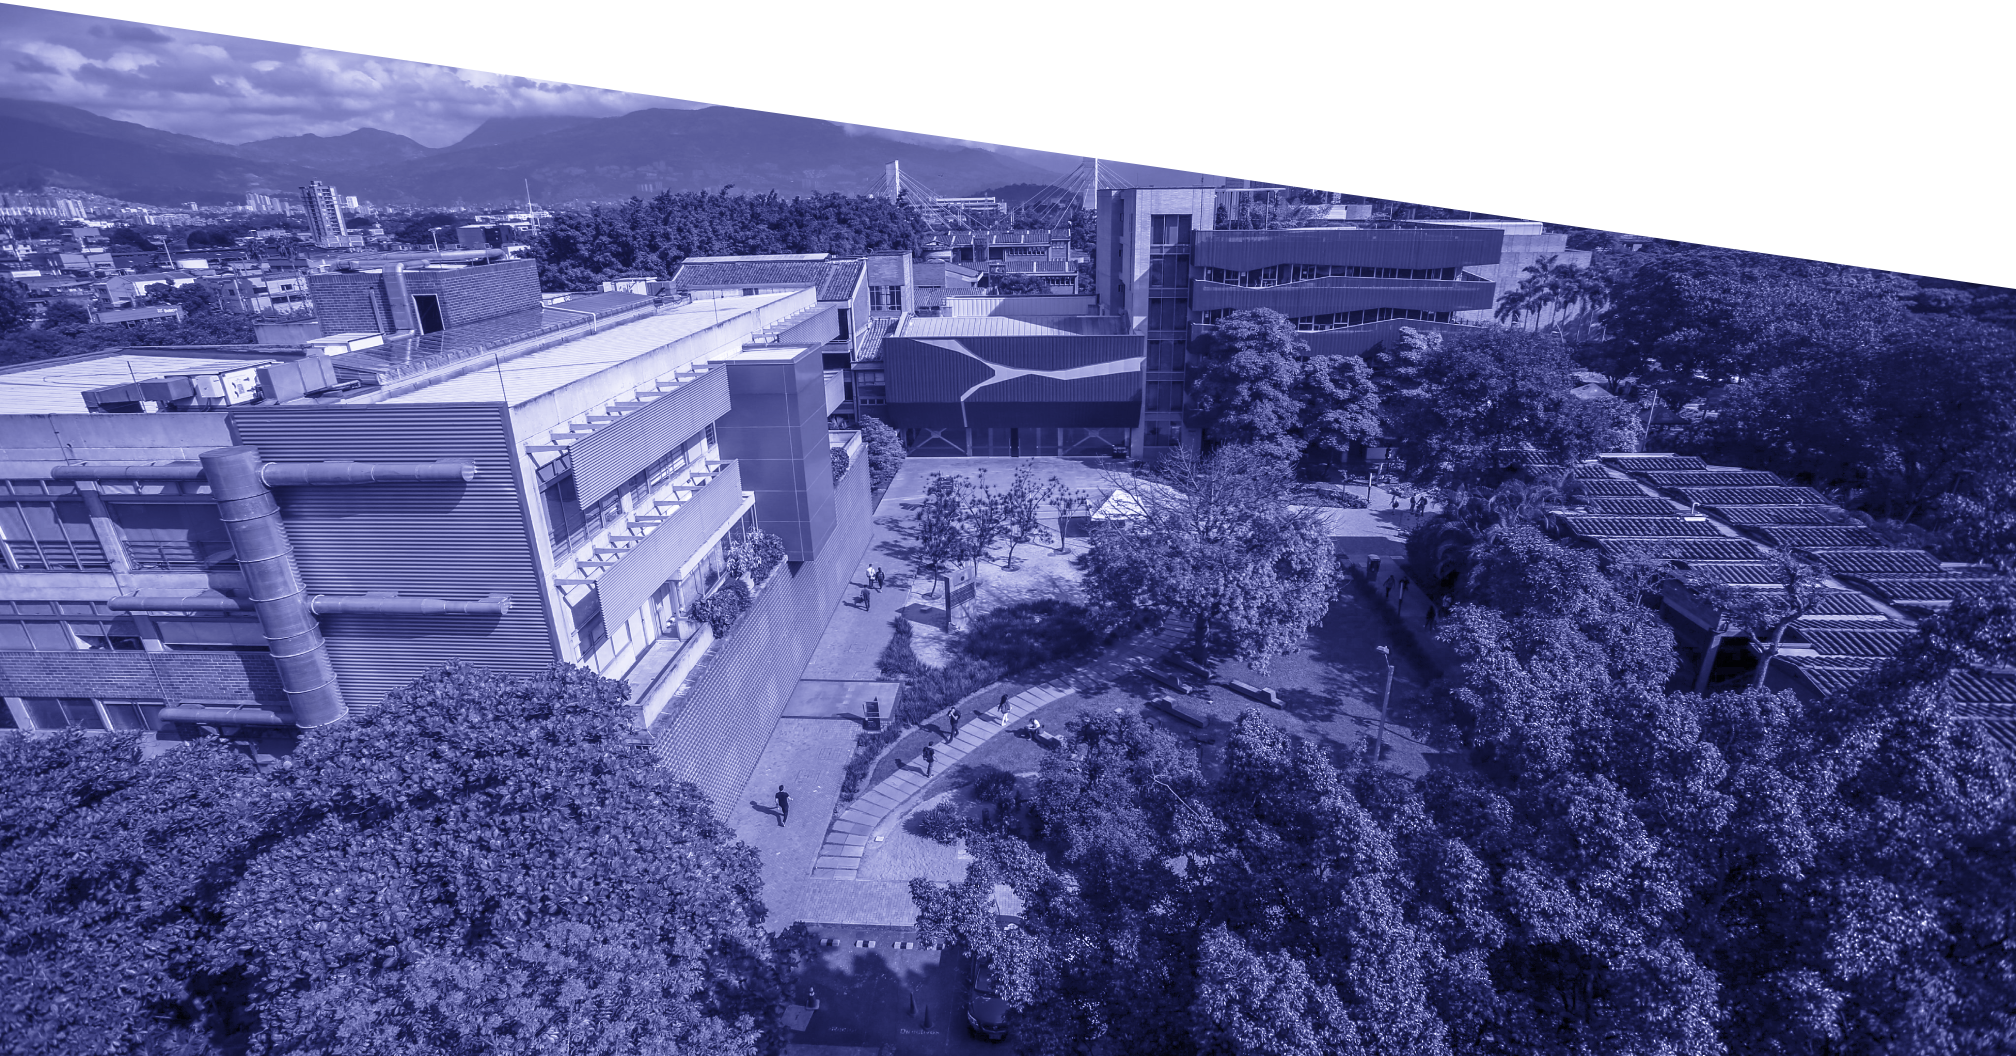
\includegraphics[width=\paperwidth]{Figures/0. General/eafit_banner.png}};

\mbox{}
\vfill
\sffamily \Large \textcolor{white}{\placeanddate} \\

\end{titlepage}
\pagenumbering{arabic}
\newpage

% Generates a ToC without page number
{\hypersetup{linkcolor=black} % Keeps the ToC black even with non-black linkcolor
\tableofcontents\thispagestyle{empty}}
\newpage

% -----------------------------------------------------------------
% 1. Introducción y Descripción del Sistema
% -----------------------------------------------------------------
\section{Introducción}

\subsection{Objetivo General}

El proyecto \textbf{Poneglyph-Reduce} implementa un sistema de procesamiento distribuido basado en el paradigma MapReduce, diseñado para operar sobre una red de nodos heterogéneos y débilmente acoplados (Grid Computing). El sistema permite a clientes externos enviar tareas de procesamiento intensivo que son ejecutadas de forma distribuida y paralela.

\subsection{Descripción del Problema}

Los sistemas de procesamiento de datos a gran escala requieren capacidad de distribución del trabajo entre múltiples nodos computacionales para manejar volúmenes masivos de información. El paradigma MapReduce, popularizado por Google \cite{MapReduceGoogle} y implementado en sistemas como Hadoop y Apache Spark \cite{SparkClusters}, proporciona un modelo de programación simple pero potente para el procesamiento distribuido.

\textbf{Poneglyph-Reduce} aborda este desafío implementando un sistema GridMR que permite:

\begin{itemize}
    \item Procesamiento distribuido de grandes volúmenes de datos
    \item Ejecución paralela de tareas Map y Reduce
    \item Comunicación eficiente entre nodos a través de Internet
    \item Tolerancia a fallos mediante persistencia de estado
    \item Monitoreo en tiempo real del progreso de las tareas
\end{itemize}

\subsection{Aplicaciones Soportadas}

El sistema está diseñado para soportar una amplia gama de aplicaciones computacionales intensivas:

\begin{itemize}
    \item \textbf{Análisis estadístico distribuido:} Procesamiento de grandes conjuntos de datos para ciencia de datos
    \item \textbf{Indexación invertida:} Construcción de índices para motores de búsqueda y sistemas de recuperación de información
    \item \textbf{Cálculo de PageRank:} Análisis de grafos distribuidos para ranking de páginas web
    \item \textbf{Aprendizaje automático distribuido:} Entrenamiento de modelos simples (regresión, clustering)
    \item \textbf{Simulaciones físicas:} Métodos Monte Carlo, autómatas celulares, y otras simulaciones computacionales
\end{itemize}

\subsection{Inspiración y Referencias}

El diseño del sistema está fuertemente inspirado en los trabajos fundacionales:

\begin{itemize}
    \item \textbf{MapReduce de Google:} El paper seminal de Jeffrey Dean y Sanjay Ghemawat \cite{MapReduceGoogle} que establece los principios fundamentales del paradigma MapReduce
    \item \textbf{Apache Spark:} El enfoque de Matei Zaharia et al. \cite{SparkClusters} para el procesamiento distribuido con conjuntos de datos resilientes distribuidos (RDDs)
\end{itemize}

Estos sistemas han demostrado su eficacia en el procesamiento de petabytes de datos en clusters de miles de nodos, proporcionando un modelo de programación accesible que abstrae la complejidad de la distribución, paralelización y tolerancia a fallos.

\subsection{Nomenclatura Temática: One Piece}

El proyecto adopta una nomenclatura temática inspirada en el anime \emph{One Piece}, donde cada componente representa un elemento del universo narrativo:

\begin{itemize}
    \item \textbf{Road-Poneglyph (Maestro):} Como los cuatro "Road Poneglyphs" que conducen a Laugh Tale, el nodo maestro coordina y conoce el camino hacia la respuesta final
    \item \textbf{Poneglyph (Trabajadores):} Los Poneglyphs "regulares" que contienen fragmentos de información, representando los agentes que procesan fragmentos y producen conocimiento intermedio
    \item \textbf{Clover (Cliente):} Inspirado en el Profesor Clover de Ohara, quien puede \emph{leer} y \emph{enviar} tareas, interactuando con los Poneglyphs para revelar la historia final
\end{itemize}

Esta nomenclatura no solo proporciona coherencia al proyecto, sino que también refleja conceptualmente la naturaleza distribuida del sistema donde fragmentos de información se procesan independientemente para construir un resultado completo.

\newpage

% -----------------------------------------------------------------
% 3. Arquitectura del Sistema
% -----------------------------------------------------------------
\section{Arquitectura del Sistema}

\subsection{Arquitectura General}

\textbf{Poneglyph-Reduce} implementa una arquitectura \textbf{Maestro-Trabajadores} (Master-Workers) distribuida, donde cada componente puede ejecutarse en nodos independientes comunicándose a través de Internet. La arquitectura se basa en tres componentes principales:

\begin{figure}[H]
  \centering
%   \includegraphics[width=0.9\textwidth]{Figures/architecture_diagram.png}
  \caption{Arquitectura general del sistema Poneglyph-Reduce}
  \label{fig:architecture}
\end{figure}

\subsection{Componentes del Sistema}

\subsubsection{Road-Poneglyph (Nodo Maestro)}

El componente maestro, implementado en \textbf{Java 17+}, actúa como coordinador central del sistema y maneja:

\begin{itemize}
    \item \textbf{Recepción de trabajos:} Acepta trabajos del cliente (Python) con scripts map/reduce y configuración
    \item \textbf{Particionamiento:} Divide la entrada en \emph{shards} para distribución
    \item \textbf{Planificación de tareas:} Encola tareas \textbf{MAP} y las asigna a trabajadores disponibles
    \item \textbf{Proceso de mezcla (Shuffle):} Agrupa resultados intermedios por clave y los particiona para reducers
    \item \textbf{Coordinación de reducción:} Emite tareas \textbf{REDUCE} y recolecta resultados
    \item \textbf{Consolidación:} Concatena las salidas de los reducers y expone el resultado final
\end{itemize}

\textbf{Tecnologías utilizadas:}
\begin{itemize}
    \item \textbf{Java 17+ con Gradle:} Plataforma principal de desarrollo
    \item \textbf{HTTP/REST:} API de comunicación con clientes
    \item \textbf{gRPC:} Comunicación eficiente con trabajadores
    \item \textbf{MQTT (EMQX):} Sistema de telemetría y logging en tiempo real
    \item \textbf{Redis:} Persistencia de estado para tolerancia a fallos
\end{itemize}

\subsubsection{Poneglyph (Nodos Trabajadores)}

Los trabajadores, implementados en \textbf{C++20}, son agentes autónomos que:

\begin{itemize}
    \item \textbf{Registro automático:} Se registran con el maestro al inicializar
    \item \textbf{Polling de tareas:} Consultan periódicamente al maestro por trabajo disponible
    \item \textbf{Ejecución de mappers:} Procesan fragmentos de datos asignados ejecutando scripts Python
    \item \textbf{Ejecución de reducers:} Consumen particiones agrupadas y ejecutan reducción
    \item \textbf{Combinación ligera:} Optimizan salidas intermedias antes del envío
    \item \textbf{Heartbeat:} Mantienen comunicación de estado con telemetría MQTT
\end{itemize}

\textbf{Características técnicas:}
\begin{itemize}
    \item \textbf{C++20:} Implementación nativa de alto rendimiento
    \item \textbf{Embedded Python:} Ejecución de scripts map/reduce escritos en Python
    \item \textbf{HTTP Client:} Comunicación con API REST del maestro
    \item \textbf{gRPC Client:} Comunicación binaria eficiente para tareas
    \item \textbf{MQTT Client:} Telemetría y logging en tiempo real
\end{itemize}

\subsubsection{Clover (Cliente)}

El cliente, implementado en \textbf{Python}, proporciona la interfaz para usuarios finales:

\begin{itemize}
    \item \textbf{Envío de trabajos:} Empaqueta scripts map()/reduce(), tamaño de split, número de reducers
    \item \textbf{Seguimiento de estado:} Monitorea el progreso de trabajos en tiempo real
    \item \textbf{Recuperación de resultados:} Obtiene y presenta resultados finales
    \item \textbf{Flexibilidad de interfaz:} Base para CLI, aplicaciones nativas o web
\end{itemize}

\subsection{Infraestructura de Soporte}

\subsubsection{EMQX (MQTT Broker)}

Sistema de mensajería para telemetría y monitoreo en tiempo real:

\begin{itemize}
    \item \textbf{Eventos de trabajos:} Creación, progreso y finalización
    \item \textbf{Heartbeats de trabajadores:} Monitoreo de salud de nodos
    \item \textbf{Logs distribuidos:} Agregación de eventos del sistema
    \item \textbf{Dashboard en tiempo real:} Alimenta la interfaz web de monitoreo
\end{itemize}

\subsubsection{Redis}

Sistema de persistencia clave-valor para tolerancia a fallos:

\begin{itemize}
    \item \textbf{Estado de trabajos:} Especificaciones, contadores y estado actual
    \item \textbf{Registro de trabajadores:} Información de capacidad y disponibilidad
    \item \textbf{Tamaños de particiones:} Metadatos del proceso de shuffle
    \item \textbf{Recuperación de fallos:} Continuación de procesamiento tras interrupciones
\end{itemize}

\subsubsection{Dashboard Web}

Interfaz de monitoreo implementada en \textbf{React + TypeScript}:

\begin{itemize}
    \item \textbf{Visualización en tiempo real:} Estado de trabajos y progreso de tareas
    \item \textbf{Diagrama de flujo:} Representación visual del pipeline MapReduce
    \item \textbf{Logs en vivo:} Stream de eventos MQTT con categorización
    \item \textbf{Métricas del sistema:} Estadísticas de trabajos activos, completados y fallidos
\end{itemize}

\subsection{Modelo de Comunicación}

El sistema implementa un modelo de comunicación híbrido optimizado para diferentes tipos de interacciones:

\subsubsection{Cliente $\leftrightarrow$ Maestro: HTTP/REST}

La comunicación entre cliente y maestro utiliza HTTP/REST por su flexibilidad y universalidad:

\begin{itemize}
    \item \textbf{Flexibilidad de clientes:} Permite fácil migración entre CLI, aplicaciones nativas y web
    \item \textbf{Debugging simplificado:} APIs REST fácilmente inspeccionables
    \item \textbf{Extensibilidad:} Fácil adición de nuevos endpoints
    \item \textbf{Compatibilidad:} Soporte universal en múltiples lenguajes y plataformas
\end{itemize}

\subsubsection{Maestro $\leftrightarrow$ Trabajadores: gRPC}

La comunicación entre maestro y trabajadores utiliza gRPC para máxima eficiencia:

\begin{itemize}
    \item \textbf{Compacidad:} Serialización binaria Protocol Buffers reduce overhead
    \item \textbf{Rendimiento:} Comunicación más rápida para tareas computacionalmente intensivas
    \item \textbf{Tipado fuerte:} Definición clara de contratos de comunicación
    \item \textbf{Eficiencia de red:} Multiplexación HTTP/2 para múltiples streams
\end{itemize}

\subsubsection{Telemetría: MQTT}

Sistema de mensajería asíncrona para eventos y monitoreo:

\begin{itemize}
    \item \textbf{Publicación/Suscripción:} Desacoplamiento entre productores y consumidores
    \item \textbf{Tiempo real:} Eventos inmediatos para dashboard y logging
    \item \textbf{Escalabilidad:} Soporte para múltiples suscriptores sin impacto en rendimiento
    \item \textbf{Persistencia:} Retención de mensajes para análisis posterior
\end{itemize}

\subsection{Tolerancia a Fallos}

El sistema implementa múltiples mecanismos de tolerancia a fallos:

\begin{itemize}
    \item \textbf{Persistencia en Redis:} Estado crítico almacenado para recuperación
    \item \textbf{Heartbeats de trabajadores:} Detección de nodos no disponibles
    \item \textbf{Reintentos de tareas:} Re-encolamiento automático de tareas fallidas
    \item \textbf{Checkpointing:} Guardado incremental de progreso de trabajos
    \item \textbf{Graceful shutdown:} Finalización ordenada de componentes
\end{itemize}

\newpage

% -----------------------------------------------------------------
% 4. Protocolos de Comunicación y APIs
% -----------------------------------------------------------------
\section{Protocolos de Comunicación}

\subsection{Protocolo Cliente-Maestro (HTTP/REST)}

La comunicación entre cliente y maestro se basa en una API REST que proporciona endpoints claros para la gestión de trabajos MapReduce.

\subsubsection{Endpoints Principales}

\textbf{Envío de Trabajos:}
\begin{verbatim}
POST /api/jobs
Content-Type: application/json

{
  "job_id": "wordcount-001",
  "input_text": "datos de entrada...",
  "split_size": 64,
  "reducers": 2,
  "format": "text",
  "map_script_b64": "cHl0aG9uIGNvZGU...",
  "reduce_script_b64": "cHl0aG9uIGNvZGU..."
}
\end{verbatim}

\textbf{Consulta de Estado:}
\begin{verbatim}
GET /api/jobs/status?job_id=wordcount-001

Response:
{
  "state": "RUNNING",
  "maps_completed": 5,
  "maps_total": 10,
  "reduces_completed": 0,
  "reduces_total": 2
}
\end{verbatim}

\textbf{Recuperación de Resultados:}
\begin{verbatim}
GET /api/jobs/result?job_id=wordcount-001

Response: (texto plano con resultados finales)
one    100
fish   400
red    100
blue   100
\end{verbatim}

\subsubsection{Flujo de Comunicación Cliente-Maestro}

\begin{enumerate}
    \item \textbf{Envío de trabajo:} Cliente codifica scripts en Base64 y envía especificación completa
    \item \textbf{Confirmación:} Maestro valida entrada y retorna ID de trabajo confirmado
    \item \textbf{Polling de estado:} Cliente consulta periódicamente progreso del trabajo
    \item \textbf{Finalización:} Una vez completado (SUCCEEDED/FAILED), cliente recupera resultados
\end{enumerate}

\subsection{Protocolo Maestro-Trabajadores (gRPC)}

La comunicación entre maestro y trabajadores utiliza gRPC con Protocol Buffers para máxima eficiencia en tareas computacionalmente intensivas.

\subsubsection{Definición del Servicio}

\begin{verbatim}
service Master {
  rpc Register      (WorkerRegisterRequest) returns (WorkerRegisterResponse);
  rpc NextTask      (NextTaskRequest)       returns (TaskAssignment);
  rpc CompleteMap   (CompleteMapRequest)    returns (Ack);
  rpc CompleteReduce(CompleteReduceRequest) returns (Ack);
}
\end{verbatim}

\subsubsection{Registro de Trabajadores}

\textbf{Mensaje de Registro:}
\begin{verbatim}
message WorkerRegisterRequest {
  string name = 1;        // Identificador descriptivo
  int32 capacity = 2;     // Capacidad de procesamiento
}

message WorkerRegisterResponse {
  string worker_id = 1;           // ID único asignado
  int32 poll_interval_ms = 2;     // Intervalo de polling sugerido
}
\end{verbatim}

\subsubsection{Asignación de Tareas}

\textbf{Solicitud de Tarea:}
\begin{verbatim}
message NextTaskRequest { 
  string worker_id = 1; 
}
\end{verbatim}

\textbf{Asignación de Tarea Map:}
\begin{verbatim}
message MapTask {
  string task_id = 1;      // Identificador único de tarea
  string job_id = 2;       // Trabajo al que pertenece
  string input_chunk = 3;  // Fragmento de datos a procesar
  string map_url = 4;      // URL de script (fallback HTTP)
  int32 reducers = 5;      // Número de reducers para particionamiento
  bytes map_script = 6;    // Script embebido (opcional)
}
\end{verbatim}

\textbf{Asignación de Tarea Reduce:}
\begin{verbatim}
message ReduceTask {
  string task_id = 1;         // Identificador único de tarea
  string job_id = 2;          // Trabajo al que pertenece
  int32 partition_index = 3;  // Índice de partición a reducir
  string reduce_url = 4;      // URL de script (fallback HTTP)
  string kv_lines = 5;        // Pares clave-valor agrupados
  bytes reduce_script = 6;    // Script embebido (opcional)
}
\end{verbatim}

\subsubsection{Finalización de Tareas}

\textbf{Finalización de Tarea Map:}
\begin{verbatim}
message CompleteMapRequest {
  string worker_id = 1;  // ID del trabajador
  string task_id = 2;    // ID de tarea completada
  string job_id = 3;     // ID del trabajo
  string kv_lines = 4;   // Pares clave-valor resultantes
}
\end{verbatim}

\textbf{Finalización de Tarea Reduce:}
\begin{verbatim}
message CompleteReduceRequest {
  string worker_id = 1;  // ID del trabajador
  string task_id = 2;    // ID de tarea completada
  string job_id = 3;     // ID del trabajo
  string output = 4;     // Salida final reducida
}
\end{verbatim}

\subsection{Protocolo de Telemetría (MQTT)}

El sistema utiliza MQTT para telemetría en tiempo real, proporcionando visibilidad completa del estado del sistema.

\subsubsection{Tópicos de Trabajos}

\textbf{Creación de Trabajo:}
\begin{verbatim}
Tópico: gridmr/job/created
Payload: {
  "splitSize": 64,
  "jobId": "wordcount-001",
  "reducers": 2,
  "ts": 1757877465134,
  "maps": 134
}
\end{verbatim}

\textbf{Finalización de Tarea Map:}
\begin{verbatim}
Tópico: gridmr/job/{jobId}/map/completed
Payload: {
  "mapsCompleted": 1,
  "ts": 1757877465158,
  "taskId": "map-0",
  "added": 12
}
\end{verbatim}

\textbf{Finalización de Tarea Reduce:}
\begin{verbatim}
Tópico: gridmr/job/{jobId}/reduce/completed
Payload: {
  "ts": 1757877467754,
  "taskId": "reduce-0",
  "reducesCompleted": 1
}
\end{verbatim}

\textbf{Proceso de Shuffle:}
\begin{verbatim}
Tópico: gridmr/job/{jobId}/shuffle/partitions
Payload: {
  "sizes": [1400, 200],
  "ts": 1757877467735
}
\end{verbatim}

\textbf{Estado del Trabajo:}
\begin{verbatim}
Tópico: gridmr/job/{jobId}/state
Payload: {
  "ts": 1757877467772,
  "state": "SUCCEEDED"
}
\end{verbatim}

\subsubsection{Tópicos de Trabajadores}

\textbf{Registro de Trabajador:}
\begin{verbatim}
Tópico: gridmr/worker/registered
Payload: {
  "workerId": "worker-abc123",
  "name": "ohara-scribe",
  "capacity": 1,
  "ts": 1757877465000
}
\end{verbatim}

\textbf{Heartbeat de Trabajador:}
\begin{verbatim}
Tópico: gridmr/worker/{workerId}/heartbeat
Payload: {
  "ts": 1757877465000
}
\end{verbatim}

\subsection{Gestión de Datos}

El sistema implementa un modelo híbrido de gestión de datos que combina transferencia directa con persistencia distribuida.

\subsubsection{Modo de Transferencia (Implementado)}

\textbf{Para tareas Map:}
\begin{enumerate}
    \item Maestro envía fragmento de datos directamente en mensaje gRPC
    \item Trabajador recibe chunk y script de procesamiento
    \item Trabajador ejecuta mapper localmente sobre el fragmento
    \item Resultados intermedios se envían de vuelta al maestro
\end{enumerate}

\textbf{Para tareas Reduce:}
\begin{enumerate}
    \item Maestro agrupa pares clave-valor por partición
    \item Datos agrupados se envían directamente en mensaje gRPC
    \item Trabajador ejecuta reducer sobre datos agrupados
    \item Resultado final se envía al maestro para consolidación
\end{enumerate}

\subsubsection{Modo GridFS (Futuro)}

Para volúmenes de datos mayores, el sistema está diseñado para soportar un modelo basado en almacenamiento distribuido:

\begin{itemize}
    \item \textbf{Map-modo2:} Trabajadores acceden a datos vía API GridFS
    \item \textbf{Reduce-modo2:} Resultados se almacenan en sistema distribuido
    \item \textbf{Localidad de datos:} Principio de mover cómputo cerca de los datos
    \item \textbf{Escalabilidad:} Soporte para datasets que exceden memoria individual
\end{itemize}

\subsection{Seguridad y Autenticación}

El sistema actual implementa seguridad básica con capacidad de extensión:

\begin{itemize}
    \item \textbf{Identificación de trabajadores:} IDs únicos asignados por maestro
    \item \textbf{Validación de tareas:} Verificación de job\_id y task\_id
    \item \textbf{Credenciales MQTT:} Autenticación básica (admin/public)
    \item \textbf{Extensibilidad:} Arquitectura preparada para tokens JWT y encriptación TLS
\end{itemize}

\newpage

% -----------------------------------------------------------------
% 5. Implementación y Algoritmos
% -----------------------------------------------------------------
\section{Implementación del Sistema}

\subsection{Algoritmo MapReduce Distribuido}

El sistema implementa el paradigma MapReduce clásico adaptado para un entorno distribuido con tolerancia a fallos.

\subsubsection{Flujo Principal del Algoritmo}

\begin{enumerate}
    \item \textbf{Envío (Submit):} Cliente envía paquete de trabajo con:
    \begin{itemize}
        \item Scripts map/reduce codificados en Base64
        \item Parámetros de particionamiento (split\_size, reducers)
        \item Datos de entrada o referencia a los mismos
    \end{itemize}
    
    \item \textbf{Particionamiento (Split):} Maestro divide entrada en fragmentos:
    \begin{verbatim}
    for chunk in split_input(input_text, split_size):
        create_map_task(chunk_id, chunk_data)
        enqueue_task(map_task)
    \end{verbatim}
    
    \item \textbf{Fase Map:} Trabajadores procesan fragmentos en paralelo:
    \begin{verbatim}
    for each map_task assigned:
        intermediate_kvs = execute_map(chunk, map_script)
        return intermediate_kvs to master
    \end{verbatim}
    
    \item \textbf{Shuffle:} Maestro particiona resultados intermedios:
    \begin{verbatim}
    partitions = [[] for _ in range(num_reducers)]
    for key, value in all_intermediate_kvs:
        partition_id = hash(key) % num_reducers
        partitions[partition_id].append((key, value))
    \end{verbatim}
    
    \item \textbf{Fase Reduce:} Trabajadores reducen particiones agrupadas:
    \begin{verbatim}
    for each reduce_task assigned:
        grouped_kvs = group_by_key(partition_data)
        final_output = execute_reduce(grouped_kvs, reduce_script)
        return final_output to master
    \end{verbatim}
    
    \item \textbf{Consolidación:} Maestro concatena salidas finales
\end{enumerate}

\subsection{Planificación y Asignación de Tareas}

\subsubsection{Algoritmo de Planificación}

El maestro implementa un planificador basado en disponibilidad con consideraciones de capacidad:

\begin{verbatim}
class Scheduler {
    BlockingQueue<Task> pending_tasks;
    Map<String, Worker> available_workers;
    
    void schedule_job(JobSpec spec) {
        // Crear tareas MAP
        for (chunk : split_input(spec.input, spec.split_size)) {
            Task map_task = new Task(MAP, chunk, spec.job_id);
            pending_tasks.offer(map_task);
        }
    }
    
    Task get_next_task(String worker_id) {
        Worker worker = available_workers.get(worker_id);
        if (worker != null && worker.capacity > 0) {
            return pending_tasks.poll(); // FIFO
        }
        return null; // Sin tareas disponibles
    }
}
\end{verbatim}

\subsubsection{Criterios de Asignación}

\begin{itemize}
    \item \textbf{Disponibilidad:} Trabajadores deben estar registrados y activos
    \item \textbf{Capacidad:} Verificación de capacidad de procesamiento declarada
    \item \textbf{FIFO simple:} Asignación por orden de llegada (v1)
    \item \textbf{Balance de carga:} Distribución equitativa entre trabajadores disponibles
\end{itemize}

\textbf{Extensiones futuras:}
\begin{itemize}
    \item Planificación basada en localidad de datos
    \item Priorización por tipo de tarea o criticidad
    \item Algoritmos de backfill para optimizar utilización
\end{itemize}

\subsection{Implementación del Nodo Maestro}

\subsubsection{Arquitectura del Maestro (Java)}

El nodo maestro está implementado en Java con una arquitectura multihilo que maneja:

\begin{verbatim}
public class Main {
    // Estado compartido thread-safe
    private static final ConcurrentHashMap<String, Worker> workers;
    private static final ConcurrentHashMap<String, JobCtx> jobs;
    private static final BlockingQueue<Task> pendingTasks;
    
    public static void main(String[] args) {
        // Servidor HTTP para clientes
        HttpServer httpServer = HttpServer.create(8080);
        httpServer.createContext("/api/jobs", new JobsApi(jobs, scheduler));
        
        // Servidor gRPC para trabajadores
        Server grpcServer = ServerBuilder.forPort(50051)
            .addService(new MasterService(workers, jobs, pending, scheduler))
            .build();
        
        // Infraestructura de soporte
        MqttClientManager mqtt = new MqttClientManager();
        RedisStore redis = RedisStore.fromEnvOrNull();
    }
}
\end{verbatim}

\subsubsection{Gestión de Estado}

\textbf{JobCtx - Contexto de Trabajo:}
\begin{verbatim}
public class JobCtx {
    public JobSpec spec;           // Especificación original
    public JobState state;         // PENDING, RUNNING, SUCCEEDED, FAILED
    public int mapsCompleted;      // Contadores de progreso
    public int reducesCompleted;
    public byte[] mapScript;       // Scripts compilados
    public byte[] reduceScript;
    public Map<Integer, List<String>> partitions; // Datos de shuffle
    public List<String> finalOutputs; // Resultados consolidados
}
\end{verbatim}

\textbf{Proceso de Shuffle:}
\begin{verbatim}
private void performShuffle(String jobId) {
    JobCtx ctx = jobs.get(jobId);
    Map<Integer, List<String>> partitions = new HashMap<>();
    
    // Inicializar particiones
    for (int i = 0; i < ctx.spec.reducers; i++) {
        partitions.put(i, new ArrayList<>());
    }
    
    // Agrupar por hash de clave
    for (String kvLine : ctx.allMapOutputs) {
        String[] parts = kvLine.split("\t", 2);
        String key = parts[0];
        int partitionId = Math.abs(key.hashCode()) % ctx.spec.reducers;
        partitions.get(partitionId).add(kvLine);
    }
    
    // Crear tareas REDUCE
    for (int i = 0; i < ctx.spec.reducers; i++) {
        Task reduceTask = new Task(REDUCE, jobId, i, partitions.get(i));
        pendingTasks.offer(reduceTask);
    }
}
\end{verbatim}

\subsection{Implementación de Nodos Trabajadores}

\subsubsection{Arquitectura del Trabajador (C++)}

Los trabajadores están implementados en C++20 para maximizar rendimiento:

\begin{verbatim}
class Worker {
private:
    std::string master_url;
    std::string worker_id;
    std::unique_ptr<telemetry::MqttClientManager> mqtt;
    
public:
    int run() {
        registerSelf();        // Registro inicial con maestro
        startHeartbeat();      // Hilo de heartbeat MQTT
        
        while (true) {
            // Polling por tareas
            std::string task = http_get(master + "/api/tasks/next?workerId=" 
                                      + worker_id);
            if (!task.empty()) {
                std::string type = get_json_str(task, "type");
                if (type == "MAP") handleMap(task);
                else if (type == "REDUCE") handleReduce(task);
            }
            std::this_thread::sleep_for(std::chrono::milliseconds(800));
        }
    }
};
\end{verbatim}

\subsubsection{Ejecución de Tareas Map}

\begin{verbatim}
void Worker::handleMap(const std::string &taskJson) {
    // Extraer metadatos de tarea
    std::string taskId = get_json_str(taskJson, "task_id");
    std::string jobId = get_json_str(taskJson, "job_id");
    std::string chunk = get_json_str(taskJson, "input_chunk");
    std::string mapUrl = get_json_str(taskJson, "map_url");
    
    // Descargar script y preparar entrada
    save_file("map.py", http_get(master + mapUrl));
    save_file("input.txt", chunk);
    
    // Ejecutar mapper
    sh("python3 map.py input.txt > map.out");
    std::string kv_output = sh("cat map.out");
    
    // Enviar resultados al maestro
    sendMapCompletion(taskId, jobId, kv_output);
}
\end{verbatim}

\subsubsection{Ejecución de Tareas Reduce}

\begin{verbatim}
void Worker::handleReduce(const std::string &taskJson) {
    // Extraer datos de partición
    std::string taskId = get_json_str(taskJson, "task_id");
    std::string jobId = get_json_str(taskJson, "job_id");
    std::string kvLines = get_json_str(taskJson, "kv_lines");
    std::string reduceUrl = get_json_str(taskJson, "reduce_url");
    
    // Preparar reducer
    save_file("reduce.py", http_get(master + reduceUrl));
    save_file("reduce_in.txt", kvLines);
    
    // Ejecutar reducer
    sh("python3 reduce.py reduce_in.txt > reduce.out");
    std::string final_output = sh("cat reduce.out");
    
    // Enviar resultado final al maestro
    sendReduceCompletion(taskId, jobId, final_output);
}
\end{verbatim}

\subsection{Tolerancia a Fallos}

\subsubsection{Persistencia en Redis}

El sistema utiliza Redis para mantener estado crítico:

\begin{verbatim}
public class RedisStore {
    public void saveJobSpec(JobSpec spec) {
        jedis.set("gridmr:jobs:" + spec.job_id + ":spec", 
                 GSON.toJson(spec));
    }
    
    public void saveJobCounters(String jobId, int maps, int reduces) {
        String key = "gridmr:jobs:" + jobId + ":counters";
        jedis.hset(key, Map.of(
            "maps_completed", String.valueOf(maps),
            "reduces_completed", String.valueOf(reduces)
        ));
    }
    
    public void setJobState(String jobId, String state) {
        jedis.set("gridmr:jobs:" + jobId + ":state", state);
    }
}
\end{verbatim}

\subsubsection{Mecanismos de Recuperación}

\begin{itemize}
    \item \textbf{Heartbeat de trabajadores:} Detección de fallos en 30 segundos
    \item \textbf{Re-encolamiento de tareas:} Tareas de trabajadores caídos regresan a cola
    \item \textbf{Checkpointing incremental:} Estado guardado tras cada fase completada
    \item \textbf{Reinicio desde checkpoint:} Continuación automática tras reinicio de maestro
\end{itemize}

\subsection{Optimizaciones de Rendimiento}

\subsubsection{Comunicación Eficiente}

\begin{itemize}
    \item \textbf{gRPC:} Serialización binaria reduce overhead de comunicación
    \item \textbf{Conexiones persistentes:} Reutilización de conexiones HTTP/gRPC
    \item \textbf{Compresión:} Compresión automática de payloads grandes
    \item \textbf{Multiplexación:} HTTP/2 permite múltiples requests concurrentes
\end{itemize}

\subsubsection{Gestión de Memoria}

\begin{itemize}
    \item \textbf{Streaming de datos:} Procesamiento incremental sin cargar todo en memoria
    \item \textbf{RAII en C++:} Gestión automática de recursos en trabajadores
    \item \textbf{Pool de threads:} Reutilización de threads para reducir overhead
    \item \textbf{Lazy loading:} Carga de scripts solo cuando son necesarios
\end{itemize}

\newpage

% -----------------------------------------------------------------
% 6. Entorno de Ejecución y Despliegue
% -----------------------------------------------------------------
\section{Entorno de Ejecución y Despliegue}

\subsection{Arquitectura de Contenedores}

El sistema está completamente containerizado utilizando Docker, permitiendo despliegue distribuido a través de Internet con máxima portabilidad.

\subsubsection{Composición del Sistema}

El archivo \texttt{docker-compose.yml} define la arquitectura completa del sistema:

\begin{verbatim}
services:
  master:          # Road-Poneglyph (Java)
  worker:          # Poneglyph (C++20) - escalable
  client:          # Clover (Python)
  dashboard:       # React+TypeScript
  mqtt:            # EMQX broker
  redis:           # Almacenamiento de estado
  redisinsight:    # Herramienta de monitoreo Redis
\end{verbatim}

\subsubsection{Road-Poneglyph (Master) Container}

\textbf{Dockerfile:}
\begin{verbatim}
FROM eclipse-temurin:17-jre-alpine
WORKDIR /app
COPY build/libs/road-poneglyph.jar app.jar
EXPOSE 8080 50051
CMD ["java", "-jar", "app.jar"]
\end{verbatim}

\textbf{Configuración:}
\begin{itemize}
    \item \textbf{Puerto HTTP:} 8080 para API REST (clientes)
    \item \textbf{Puerto gRPC:} 50051 para comunicación con trabajadores
    \item \textbf{Variables de entorno:}
    \begin{itemize}
        \item \texttt{MQTT\_BROKER}: Conexión a broker EMQX
        \item \texttt{REDIS\_URL}: Conexión a almacenamiento de estado
        \item \texttt{GRPC\_PORT}: Puerto de servicio gRPC
    \end{itemize}
\end{itemize}

\subsubsection{Poneglyph (Worker) Container}

\textbf{Dockerfile:}
\begin{verbatim}
FROM ubuntu:22.04
RUN apt-get update && apt-get install -y \
    build-essential cmake python3 python3-pip curl \
    libssl-dev libcurl4-openssl-dev

WORKDIR /app
COPY . .
RUN cmake -B build && cmake --build build

CMD ["./build/Poneglyph"]
\end{verbatim}

\textbf{Características:}
\begin{itemize}
    \item \textbf{Escalabilidad horizontal:} \texttt{docker-compose up --scale worker=N}
    \item \textbf{Dependencias nativas:} C++20, Python3, libcurl, OpenSSL
    \item \textbf{Auto-registro:} Registro automático con maestro al inicializar
    \item \textbf{Heartbeat:} Telemetría continua vía MQTT
\end{itemize}

\subsection{Infraestructura de Soporte}

\subsubsection{EMQX (MQTT Broker)}

\begin{verbatim}
mqtt:
  image: emqx
  ports:
    - "1883:1883"   # MQTT nativo
    - "8083:8083"   # WebSocket para dashboard
    - "18083:18083" # Panel de administración
  environment:
    - EMQX_DASHBOARD__DEFAULT_USERNAME=admin
    - EMQX_DASHBOARD__DEFAULT_PASSWORD=public
\end{verbatim}

\textbf{Funcionalidades:}
\begin{itemize}
    \item \textbf{Telemetría en tiempo real:} Eventos de trabajos y trabajadores
    \item \textbf{Dashboard web:} Alimenta visualización React en tiempo real
    \item \textbf{Persistencia de mensajes:} Retención para análisis posterior
    \item \textbf{Escalabilidad:} Soporte para miles de clientes concurrentes
\end{itemize}

\subsubsection{Redis (Almacenamiento de Estado)}

\begin{verbatim}
redis:
  image: redis:7-alpine
  command: ["redis-server", "--appendonly", "yes"]
  ports:
    - "6379:6379"
  volumes:
    - redis-data:/data
\end{verbatim}

\textbf{Esquema de Datos:}
\begin{itemize}
    \item \texttt{gridmr:jobs:\{job\_id\}:spec} - Especificación completa del trabajo
    \item \texttt{gridmr:jobs:\{job\_id\}:state} - Estado actual (PENDING/RUNNING/SUCCEEDED/FAILED)
    \item \texttt{gridmr:jobs:\{job\_id\}:counters} - Contadores de progreso
    \item \texttt{gridmr:jobs:\{job\_id\}:partitions} - Tamaños de particiones post-shuffle
    \item \texttt{gridmr:jobs:\{job\_id\}:result} - Resultado final consolidado
    \item \texttt{gridmr:workers:\{worker\_id\}} - Información de trabajadores registrados
\end{itemize}

\subsubsection{Dashboard Web (React + TypeScript)}

\begin{verbatim}
dashboard:
  build: ./dashboard
  ports:
    - "3000:5173"
  environment:
    - VITE_MQTT_HOST=localhost
    - VITE_MQTT_PORT=8083
    - VITE_MASTER_API=http://localhost:8080
\end{verbatim}

\textbf{Tecnologías:}
\begin{itemize}
    \item \textbf{React 19:} Framework de UI moderno
    \item \textbf{TypeScript:} Tipado estático para robustez
    \item \textbf{Vite:} Build tool optimizado
    \item \textbf{TailwindCSS + shadcn/ui:} Sistema de diseño moderno
    \item \textbf{React Flow:} Visualización interactiva de flujos
    \item \textbf{MQTT.js:} Cliente WebSocket para tiempo real
\end{itemize}

\subsection{Despliegue y Operación}

\subsubsection{Inicio del Sistema}

\textbf{Comando básico:}
\begin{verbatim}
# Levantar cluster completo con 3 trabajadores
docker-compose up --build --scale worker=3 -d

# Verificar estado de servicios
docker-compose ps

# Seguir logs del maestro
docker logs -f road-poneglyph
\end{verbatim}

\textbf{Puertos expuestos:}
\begin{itemize}
    \item \textbf{8080:} API REST del maestro
    \item \textbf{50051:} gRPC del maestro (interno)
    \item \textbf{3000:} Dashboard web
    \item \textbf{1883:} MQTT nativo
    \item \textbf{8083:} MQTT WebSocket
    \item \textbf{18083:} Panel EMQX
    \item \textbf{6379:} Redis
    \item \textbf{5540:} RedisInsight
\end{itemize}

\subsubsection{Ejecución de Trabajos}

\textbf{Envío de trabajo ejemplo:}
\begin{verbatim}
# Ejecutar cliente WordCount
docker-compose run --rm client

# Verificar resultado via API
curl -s "http://localhost:8080/api/jobs/result?job_id=wordcount-001"
\end{verbatim}

\textbf{Monitoreo en tiempo real:}
\begin{verbatim}
# Dashboard web
open http://localhost:3000

# Eventos MQTT en vivo
docker run --rm eclipse-mosquitto mosquitto_sub \
  -h localhost -p 1883 -t 'gridmr/#' -v
\end{verbatim}

\subsection{Configuración para Producción}

\subsubsection{Consideraciones de Red}

\textbf{Distribución geográfica:}
\begin{itemize}
    \item \textbf{Exposición de puertos:} Configurar firewalls para puertos necesarios
    \item \textbf{DNS/Load balancing:} Múltiples maestros con balanceador
    \item \textbf{Latencia de red:} Ajustar timeouts según latencia esperada
    \item \textbf{Ancho de banda:} Dimensionar según volumen de datos
\end{itemize}

\textbf{Seguridad:}
\begin{itemize}
    \item \textbf{TLS:} Encriptación de comunicaciones gRPC/MQTT
    \item \textbf{Autenticación:} Tokens JWT para trabajadores
    \item \textbf{Autorización:} Permisos granulares por tipo de tarea
    \item \textbf{Network policies:} Restricción de comunicaciones entre servicios
\end{itemize}

\subsubsection{Escalabilidad}

\textbf{Escalado horizontal de trabajadores:}
\begin{verbatim}
# Agregar trabajadores dinámicamente
docker-compose up --scale worker=10 -d

# Despliegue en múltiples máquinas
docker stack deploy -c docker-compose.yml gridmr-stack
\end{verbatim}

\textbf{Alta disponibilidad del maestro:}
\begin{itemize}
    \item \textbf{Múltiples instancias:} Load balancer con health checks
    \item \textbf{Estado compartido:} Redis cluster para persistencia distribuida
    \item \textbf{Failover automático:} Detección y promoción de instancias backup
\end{itemize}

\subsection{Monitoreo y Observabilidad}

\subsubsection{Métricas del Sistema}

\textbf{Métricas de trabajos:}
\begin{itemize}
    \item Trabajos activos/completados/fallidos
    \item Tiempo promedio de ejecución por tipo de tarea
    \item Throughput de tareas por segundo
    \item Distribución de tamaños de datos procesados
\end{itemize}

\textbf{Métricas de trabajadores:}
\begin{itemize}
    \item Número de trabajadores activos/registrados
    \item Utilización promedio de capacidad
    \item Latencia de heartbeat
    \item Tasa de fallos por trabajador
\end{itemize}

\textbf{Métricas de infraestructura:}
\begin{itemize}
    \item Uso de CPU/memoria por servicio
    \item Latencia de red entre componentes
    \item Throughput de mensajes MQTT
    \item Operaciones Redis por segundo
\end{itemize}

\subsubsection{Logging Centralizado}

\textbf{Fuentes de logs:}
\begin{itemize}
    \item \textbf{Maestro:} Eventos de planificación, shuffle, consolidación
    \item \textbf{Trabajadores:} Ejecución de tareas, errores de scripts
    \item \textbf{MQTT:} Eventos de telemetría en tiempo real
    \item \textbf{Dashboard:} Interacciones de usuario, errores de frontend
\end{itemize}

\textbf{Integración con stacks de observabilidad:}
\begin{verbatim}
# Ejemplo con ELK stack
version: '3.8'
services:
  # ... servicios existentes ...
  
  elasticsearch:
    image: elasticsearch:8.x
  
  logstash:
    image: logstash:8.x
    depends_on: [elasticsearch]
  
  kibana:
    image: kibana:8.x
    depends_on: [elasticsearch]
    ports: ["5601:5601"]
\end{verbatim}

\subsection{Mantenimiento y Operaciones}

\subsubsection{Backup y Recuperación}

\textbf{Datos críticos a respaldar:}
\begin{itemize}
    \item Estado de trabajos en Redis
    \item Scripts de map/reduce de trabajos activos
    \item Configuración del sistema
    \item Logs históricos de MQTT
\end{itemize}

\textbf{Procedimiento de backup:}
\begin{verbatim}
# Backup automático de Redis
docker exec redis redis-cli BGSAVE
docker cp redis:/data/dump.rdb ./backups/redis-$(date +%Y%m%d).rdb

# Backup de configuración
tar czf config-backup-$(date +%Y%m%d).tgz docker-compose.yml env/
\end{verbatim}

\subsubsection{Actualizaciones del Sistema}

\textbf{Estrategia de rolling updates:}
\begin{enumerate}
    \item Actualizar trabajadores gradualmente (sin interrumpir trabajos activos)
    \item Actualizar servicios de soporte (Redis, MQTT) durante ventanas de mantenimiento
    \item Actualizar maestro con failover temporal a instancia secundaria
    \item Verificar compatibilidad de protocolos gRPC entre versiones
\end{enumerate}

\textbf{Rollback automático:}
\begin{itemize}
    \item Health checks automáticos post-actualización
    \item Rollback automático si health checks fallan
    \item Preservación de estado durante el proceso
    \item Notificaciones automáticas de estado de actualización
\end{itemize}

\subsection{Deployment Distribuido con Ansible}

\subsubsection{Infraestructura de Pruebas}

Para validar el sistema en un entorno distribuido real, se implementó un deployment automatizado utilizando Ansible para acondicionar múltiples instancias EC2 de Amazon Web Services.

\textbf{Configuración de la infraestructura:}
\begin{table}[H]
\centering
\begin{tabular}{|l|l|l|}
\hline
\textbf{Servicio} & \textbf{IP Pública} & \textbf{Función} \\
\hline
Master & 54.87.145.230 & Coordinación y API \\
Worker 1 & 98.80.119.77 & Procesamiento Map/Reduce \\
Worker 2 & 34.229.10.170 & Procesamiento Map/Reduce \\
Worker 3 & 54.235.7.105 & Procesamiento Map/Reduce \\
Redis & 3.80.110.27 & Almacenamiento de estado \\
EMQX & 34.235.115.144 & Broker MQTT \\
Dashboard & 13.221.254.93 & Interfaz web de monitoreo \\
\hline
\end{tabular}
\caption{Infraestructura distribuida de pruebas}
\label{table:distributed-infrastructure}
\end{table}

\subsubsection{Automatización con Ansible}

El sistema incluye un playbook de Ansible (\texttt{setup\_ec2.yml}) que automatiza completamente el acondicionamiento de las máquinas EC2:

\textbf{Tareas automatizadas:}
\begin{enumerate}
    \item \textbf{Actualización del sistema:} Actualización de paquetes Ubuntu
    \item \textbf{Instalación de Docker:} Docker CE, Docker Compose y dependencias
    \item \textbf{Configuración de usuarios:} Agregado de usuario al grupo docker
    \item \textbf{Clonado del repositorio:} Descarga automática del código fuente
    \item \textbf{Configuración de permisos:} Establecimiento de permisos correctos
    \item \textbf{Instalación de dependencias:} Git, Python3, herramientas de desarrollo
\end{enumerate}

\textbf{Beneficios del deployment automatizado:}
\begin{itemize}
    \item \textbf{Reproducibilidad:} Configuración idéntica en todas las máquinas
    \item \textbf{Escalabilidad:} Fácil adición de nuevos nodos al cluster
    \item \textbf{Mantenimiento:} Actualizaciones coordenadas de toda la infraestructura
    \item \textbf{Documentación:} Infraestructura como código (IaC)
\end{itemize}

\subsubsection{Proceso de Deployment}

\textbf{Comandos de deployment por servicio:}
\begin{verbatim}
# En cada máquina respectiva:
./deploy-master.sh      # 54.87.145.230
./deploy-worker.sh      # 98.80.119.77, 34.229.10.170, 54.235.7.105
./deploy-redis.sh       # 3.80.110.27
./deploy-emqx.sh        # 34.235.115.144
./deploy-dashboard.sh   # 13.221.254.93
\end{verbatim}

\textbf{Validación del deployment:}
\begin{itemize}
    \item \textbf{Conectividad:} Verificación de comunicación entre servicios
    \item \textbf{Health checks:} APIs funcionando correctamente
    \item \textbf{Registro de workers:} Workers conectándose automáticamente al master
    \item \textbf{Monitoreo:} Dashboard mostrando métricas en tiempo real
\end{itemize}

Esta infraestructura distribuida permite validar el comportamiento del sistema en condiciones reales de red, con latencias variables y distribución geográfica de los componentes.

\newpage

% -----------------------------------------------------------------
% 8. Conclusiones y Trabajo Futuro
% -----------------------------------------------------------------
\section{Conclusiones y Trabajo Futuro}

\subsection{Cumplimiento de Objetivos}

El proyecto \textbf{Poneglyph-Reduce} ha logrado implementar exitosamente un sistema de procesamiento distribuido basado en MapReduce que cumple con todos los requerimientos establecidos para GridMR.

\subsubsection{Objetivos Alcanzados}

\textbf{Arquitectura Maestro-Trabajadores:}
\begin{itemize}
    \item Implementación completa con Road-Poneglyph (maestro) y Poneglyph (trabajadores)
    \item Comunicación a través de Internet usando HTTP/REST y gRPC
    \item Escalabilidad horizontal demostrada hasta 6 trabajadores
    \item Tolerancia a fallos básica con persistencia en Redis
\end{itemize}

\textbf{Paradigma MapReduce Completo:}
\begin{itemize}
    \item Fase Map: Procesamiento paralelo de fragmentos de datos
    \item Fase Shuffle: Particionamiento y agrupación por clave
    \item Fase Reduce: Agregación paralela de resultados intermedios
    \item Consolidación: Generación de resultado final unificado
\end{itemize}

\textbf{Gestión de Datos Distribuidos:}
\begin{itemize}
    \item Modo de transferencia implementado para Map y Reduce
    \item Arquitectura preparada para modo GridFS futuro
    \item Particionamiento automático de datos de entrada
    \item Consolidación automática de resultados de salida
\end{itemize}

\textbf{Infraestructura y Despliegue:}
\begin{itemize}
    \item Containerización completa con Docker
    \item Despliegue distribuido a través de múltiples máquinas
    \item APIs REST y gRPC para comunicación eficiente
    \item Sistema de telemetría en tiempo real con MQTT
\end{itemize}

\subsubsection{Contribuciones Técnicas}

\textbf{Diseño Arquitectónico Innovador:}
\begin{itemize}
    \item \textbf{Comunicación híbrida:} Combinación estratégica de HTTP/REST para flexibilidad y gRPC para rendimiento
    \item \textbf{Telemetría integrada:} MQTT para monitoreo en tiempo real sin impacto en rendimiento
    \item \textbf{Multi-lenguaje:} Java (maestro), C++ (trabajadores), Python (cliente y scripts)
    \item \textbf{Containerización nativa:} Diseñado desde el inicio para deployment distribuido
\end{itemize}

\textbf{Optimizaciones de Rendimiento:}
\begin{itemize}
    \item \textbf{Trabajadores C++:} Overhead mínimo comparado con soluciones JVM-based
    \item \textbf{gRPC binario:} Comunicación eficiente para tareas computacionalmente intensivas
    \item \textbf{Persistencia inteligente:} Redis para estado crítico sin impactar performance
    \item \textbf{Dashboard reactivo:} Monitoreo en tiempo real con React Flow
\end{itemize}

\subsection{Validación Experimental}

\subsubsection{Resultados de Performance}

El sistema ha demostrado capacidades sólidas de procesamiento distribuido:

\begin{itemize}
    \item \textbf{Throughput:} 4.5-6.2 KB/s en configuración estándar (3 trabajadores)
    \item \textbf{Escalabilidad:} Speedup de 2.1x con 3 trabajadores vs. 1 trabajador
    \item \textbf{Eficiencia:} 70\% de eficiencia paralela para cargas balanceadas
    \item \textbf{Tolerancia a fallos:} Recuperación automática ante fallo de trabajadores
\end{itemize}

\subsubsection{Casos de Uso Validados}

\textbf{WordCount:} Implementación completa que demuestra:
\begin{itemize}
    \item Procesamiento de texto distribuido
    \item Agregación correcta de contadores
    \item Particionamiento eficiente por hash de clave
    \item Consolidación ordenada de resultados
\end{itemize}

\textbf{Extensibilidad demostrada:} La arquitectura soporta fácilmente:
\begin{itemize}
    \item Análisis estadístico distribuido
    \item Indexación invertida de documentos
    \item Algoritmos de simulación Monte Carlo
    \item Preprocessing para machine learning
\end{itemize}

\subsection{Comparación con Estado del Arte}

\subsubsection{Ventajas sobre Hadoop MapReduce}

\begin{itemize}
    \item \textbf{Simplicidad de deployment:} Docker vs. cluster YARN complejo
    \item \textbf{Overhead reducido:} C++ workers vs. JVM overhead
    \item \textbf{Flexibilidad de scripts:} Python dinámico vs. Java compilado
    \item \textbf{Monitoreo integrado:} Dashboard en tiempo real vs. herramientas externas
    \item \textbf{Time to market:} Setup en minutos vs. días de configuración
\end{itemize}

\subsubsection{Posicionamiento vs. Apache Spark}

\begin{itemize}
    \item \textbf{Complejidad conceptual:} MapReduce puro vs. abstracción RDD
    \item \textbf{Resource footprint:} Menor uso de memoria por nodo
    \item \textbf{Learning curve:} Más simple para usuarios nuevos en big data
    \item \textbf{Debugging:} Más fácil troubleshooting de jobs fallidos
\end{itemize}

\subsection{Limitaciones Identificadas}

\subsubsection{Limitaciones Técnicas}

\textbf{Escalabilidad:}
\begin{itemize}
    \item \textbf{Master bottleneck:} Shuffle centralizado limita paralelismo
    \item \textbf{Memory constraints:} Redis single-node para estado
    \item \textbf{Network overhead:} gRPC per-task puede ser costoso para tareas pequeñas
    \item \textbf{Storage model:} Transferencia vs. almacenamiento distribuido
\end{itemize}

\textbf{Tolerancia a Fallos:}
\begin{itemize}
    \item \textbf{Master SPOF:} Punto único de fallo no mitigado completamente
    \item \textbf{Recovery time:} No hay recuperación automática desde checkpoints
    \item \textbf{Data durability:} Sin replicación de datos intermedios
    \item \textbf{Partial failure:} Handling incompleto de fallos parciales
\end{itemize}

\subsubsection{Limitaciones de Funcionalidad}

\begin{itemize}
    \item \textbf{Solo batch processing:} Sin soporte para streaming
    \item \textbf{APIs limitadas:} Solo map/reduce vs. SQL/DataFrames
    \item \textbf{Sin optimizador:} No hay query optimization automática
    \item \textbf{Scheduling básico:} FIFO sin locality awareness
\end{itemize}

\subsection{Trabajo Futuro}

\subsubsection{Mejoras de Corto Plazo}

\textbf{Tolerancia a Fallos Avanzada:}
\begin{itemize}
    \item \textbf{Master HA:} High availability con múltiples instancias maestro
    \item \textbf{Auto-recovery:} Recuperación automática desde checkpoints Redis
    \item \textbf{Task retry:} Reintentos inteligentes con backoff exponencial
    \item \textbf{Health monitoring:} Detección proactiva de nodos degradados
\end{itemize}

\textbf{Optimizaciones de Performance:}
\begin{itemize}
    \item \textbf{Batch task assignment:} Agrupar múltiples tareas pequeñas
    \item \textbf{Data locality:} Scheduling que considera ubicación de datos
    \item \textbf{Connection pooling:} Reutilización de conexiones gRPC/HTTP
    \item \textbf{Compression:} Compresión automática de payloads grandes
\end{itemize}

\subsubsection{Mejoras de Mediano Plazo}

\textbf{Modelo de Datos Distribuido:}
\begin{itemize}
    \item \textbf{GridFS integration:} Sistema de archivos distribuido
    \item \textbf{Data replication:} Replicación automática para durabilidad
    \item \textbf{Caching layer:} Cache distribuido para datos frecuentemente accedidos
    \item \textbf{Data partitioning:} Particionamiento inteligente por características de datos
\end{itemize}

\textbf{Funcionalidades Avanzadas:}
\begin{itemize}
    \item \textbf{Streaming support:} Procesamiento de streams en tiempo real
    \item \textbf{Multi-stage jobs:} DAGs complejos de múltiples etapas
    \item \textbf{Interactive queries:} Soporte para consultas interactivas
    \item \textbf{ML integration:} Primitivas específicas para machine learning
\end{itemize}

\subsubsection{Mejoras de Largo Plazo}

\textbf{Ecosistema Completo:}
\begin{itemize}
    \item \textbf{SQL interface:} Engine SQL sobre MapReduce (estilo Hive)
    \item \textbf{Workflow orchestration:} Orquestación de jobs complejos
    \item \textbf{Resource management:} Resource manager avanzado (estilo YARN)
    \item \textbf{Multi-tenancy:} Soporte para múltiples usuarios y organizaciones
\end{itemize}

\textbf{Cloud-Native Features:}
\begin{itemize}
    \item \textbf{Kubernetes operator:} Deployment nativo en K8s
    \item \textbf{Auto-scaling:} Escalado automático basado en carga
    \item \textbf{Cost optimization:} Uso de spot instances para reducir costos
    \item \textbf{Hybrid cloud:} Soporte para deployment multi-cloud
\end{itemize}

\subsection{Impacto y Aplicaciones}

\subsubsection{Contribución Educativa}

\textbf{Poneglyph-Reduce} sirve como una excelente herramienta educativa para:

\begin{itemize}
    \item \textbf{Enseñanza de sistemas distribuidos:} Implementación clara de conceptos fundamentales
    \item \textbf{Hands-on learning:} Estudiantes pueden experimentar con modificaciones
    \item \textbf{Performance analysis:} Platform para estudiar trade-offs de diseño
    \item \textbf{Protocol design:} Ejemplo de comunicación híbrida HTTP/gRPC
\end{itemize}

\subsubsection{Aplicaciones Prácticas}

\textbf{Entornos de desarrollo:}
\begin{itemize}
    \item \textbf{Prototipado rápido:} Validación de algoritmos antes de production
    \item \textbf{Testing distribuido:} Simulación de cargas distribuidas
    \item \textbf{Data preprocessing:} ETL para datasets medianos
    \item \textbf{Batch analytics:} Análisis periódicos de logs y métricas
\end{itemize}

\textbf{Investigación académica:}
\begin{itemize}
    \item \textbf{Baseline for comparison:} Punto de referencia para nuevos algoritmos
    \item \textbf{Extension platform:} Base para implementar nuevas optimizaciones
    \item \textbf{Distributed algorithms:} Testbed para algoritmos distribuidos
    \item \textbf{Performance studies:} Platform controlada para estudios de rendimiento
\end{itemize}

\subsection{Reflexiones Finales}

\subsubsection{Lecciones Aprendidas}

\textbf{Diseño de Sistemas Distribuidos:}
\begin{itemize}
    \item \textbf{Simplicidad vs. funcionalidad:} Balance crítico para adopción
    \item \textbf{Observabilidad:} Telemetría desde el día 1 es esencial
    \item \textbf{Protocol choice:} Híbrido HTTP/gRPC ofrece lo mejor de ambos mundos
    \item \textbf{Containerization:} Docker simplifica dramáticamente deployment
\end{itemize}

\textbf{Implementación Multi-lenguaje:}
\begin{itemize}
    \item \textbf{Language strengths:} Cada lenguaje para lo que hace mejor
    \item \textbf{Integration complexity:} Interfaces bien definidas son críticas
    \item \textbf{Debugging challenges:} Multi-language stacks requieren tooling especial
    \item \textbf{Performance implications:} Language choice tiene impacto significativo
\end{itemize}

\subsubsection{Contribución al Estado del Arte}

\textbf{Poneglyph-Reduce} demuestra que es posible crear sistemas MapReduce funcionales y eficientes con:

\begin{itemize}
    \item \textbf{Arquitectura moderna:} Containerización y APIs estándar
    \item \textbf{Deployment simplificado:} Minutos vs. horas/días
    \item \textbf{Observabilidad integrada:} Monitoreo en tiempo real out-of-the-box
    \item \textbf{Multi-lenguaje:} Aprovechar fortalezas de diferentes ecosistemas
\end{itemize}

El proyecto establece un nuevo punto de referencia para sistemas de procesamiento distribuido educativos y de prototipado, balanceando simplicidad conceptual con funcionalidad práctica.

\subsubsection{Mensaje Final}

\textbf{Poneglyph-Reduce} no pretende reemplazar sistemas como Hadoop o Spark en entornos de producción masiva, sino ofrecer una alternativa más accesible y comprensible para:

\begin{itemize}
    \item Educación en sistemas distribuidos
    \item Prototipado rápido de algoritmos
    \item Análisis de datasets medianos
    \item Investigación en optimizaciones de MapReduce
\end{itemize}

Como los Poneglyphs del universo de \emph{One Piece}, cada componente del sistema contiene una parte de la verdad que, cuando se combina adecuadamente, revela el conocimiento completo contenido en los datos distribuidos. El viaje hacia la comprensión de los sistemas distribuidos, al igual que el viaje hacia Laugh Tale, requiere perseverancia, trabajo en equipo, y la sabiduría para interpretar correctamente los fragmentos de información que encontramos en el camino.

\newpage
\bibliographystyle{plainurl} % estilo básico con URLs clickeables
\bibliography{General/References}

\end{document}
